% ===========================================================================
% Chapitre 1 — Contexte général et cadrage du projet.
%
% Les sections 1.2 (organisme d'accueil) et 1.9 (méthodologie) contiennent les
% seuls éléments que le dépôt ne permet pas d'établir. Elles sont rédigées de
% façon à n'exiger qu'une confirmation, jamais une réécriture.
% ===========================================================================
\chapter{Contexte général et cadrage du projet}
\label{chap:context}

\section{Introduction}
\label{sec:ctx_intro}

Le recrutement occupe une place particulière dans les systèmes d'information
d'entreprise : c'est l'un des rares processus où la matière première est un
document non structuré, rédigé par une personne extérieure à l'organisation,
sans format imposé, et dont la lecture engage une décision aux conséquences
durables. Un curriculum vitæ n'est ni un formulaire ni un enregistrement de
base de données ; c'est un texte libre, dont deux candidats également
compétents produiront deux versions incomparables.

Cette caractéristique explique pourquoi l'automatisation du recrutement reste
difficile alors que d'autres processus administratifs se sont largement
informatisés. Le tri des candidatures suppose de comprendre un texte, d'en
extraire des faits — compétences, durées d'expérience, niveaux de formation —
puis de les confronter à des exigences elles-mêmes exprimées en langage
naturel.

Ce chapitre présente l'environnement du projet, analyse le problème général,
étudie les solutions existantes du marché, définit le positionnement de
PIQBIT, énonce les objectifs et le périmètre, et expose la méthodologie de
conduite retenue.

\section{Organisme d'accueil et environnement du projet}
\label{sec:host_organization}

Ce projet a été réalisé au sein de \reportHostOrg, dans le cadre du projet de
fin d'études du \reportDegree{} de \reportInstitution, spécialité
\reportSpecialty, pour l'année universitaire \reportAcademicYear.

\champARemplir{Décrire ici l'organisme d'accueil en un paragraphe : secteur
d'activité, taille, positionnement, et le lien entre son activité et le sujet
traité. Si une clause de confidentialité s'applique, l'indiquer explicitement
et rester au niveau du secteur.}

Le travail a porté sur la conception et la réalisation de PIQBIT, une
plateforme destinée aux équipes de ressources humaines ayant à traiter un
volume significatif de candidatures. L'environnement technique retenu associe
une application web Angular~\cite{angular}, une interface de programmation
FastAPI en Python~\cite{fastapi}, une base PostgreSQL~\cite{postgresql} dotée
d'une extension vectorielle~\cite{pgvector}, un cache Redis, un moteur
d'autorisation externalisé~\cite{casbin} et un module d'apprentissage
automatique dédié à la prédiction salariale.

\section{Contexte général}
\label{sec:general_context}

La diffusion des offres d'emploi sur des plateformes grand public a modifié
l'équilibre du recrutement. Publier une annonce coûte désormais peu et
l'expose à un vivier large ; recevoir les candidatures coûte peu également.
En revanche, \emph{les lire} coûte autant qu'avant. Le goulot d'étranglement
s'est déplacé de la collecte vers l'analyse.

Face à cette asymétrie, les organisations adoptent des stratégies dont aucune
n'est satisfaisante. Certaines limitent la diffusion pour contenir le volume,
au prix d'un appauvrissement du vivier. D'autres appliquent des filtres
automatiques sur mots-clés, rapides mais grossiers. D'autres encore
externalisent la présélection, ce qui déplace le coût sans améliorer la
qualité du jugement.

À cette difficulté de volume s'ajoute une exigence croissante de
justification. Un candidat écarté peut demander pourquoi ; une organisation
doit pouvoir répondre autrement que par « l'outil ne vous a pas retenu ». Un
système de recrutement qui automatise sans expliquer transfère un risque à
l'organisation qui l'emploie.

Le contexte impose donc une double contrainte, et c'est cette double contrainte
qui fait l'intérêt du sujet : traiter du volume \emph{et} produire une
décision explicable. Un système qui ne satisfait que la première est un filtre
opaque ; un système qui ne satisfait que la seconde est une lecture manuelle
assistée.

\section{Étude de l'existant}
\label{sec:existing_solutions}

Plusieurs familles d'outils occupent le marché du recrutement assisté. Le
tableau~\ref{tab:existing_solutions} compare les principales catégories et les
limites qui ont motivé PIQBIT.

\begin{table}[htbp]
  \centering
  \caption{Analyse comparative des catégories de solutions de recrutement}
  \label{tab:existing_solutions}
  \begin{tabularx}{\textwidth}{L{3.3cm} L{4.5cm} X}
    \toprule
    \textbf{Catégorie} & \textbf{Forces observées} & \textbf{Limites motivant PIQBIT} \\
    \midrule
    Systèmes de suivi des candidatures
      & Cycle de vie des dossiers, historique, collaboration entre recruteurs
      & Stockent le CV sans en analyser le contenu ; le tri reste entièrement manuel \\
    Filtres par mots-clés
      & Mise en œuvre immédiate, coût nul
      & Écartent un profil dès que sa formulation diffère de l'annonce ; aucun signal n'indique la perte \\
    Jobboards avec présélection
      & Vivier large, diffusion simple
      & Critères de tri opaques, non paramétrables, non auditables par l'employeur \\
    Analyseurs de CV spécialisés
      & Extraction structurée de qualité
      & Vendus isolément : l'extraction n'est reliée ni à la notation, ni au reste du processus \\
    Assistants génératifs généralistes
      & Grande souplesse de lecture du langage
      & Réponse non ancrée dans le dossier réel ; rien ne distingue un fait extrait d'une plausibilité produite \\
    Suites RH intégrées
      & Couverture fonctionnelle étendue
      & Coût et complexité de déploiement élevés ; personnalisation de la notation souvent impossible \\
    \bottomrule
  \end{tabularx}
\end{table}

Cette étude met en évidence une discontinuité : les outils qui \emph{lisent}
le CV ne \emph{décident} pas, et ceux qui décident ne lisent pas. Entre
l'extraction structurée et la gestion du cycle de vie, la notation explicable
reste un espace peu couvert par les solutions accessibles.

PIQBIT ne cherche pas à reproduire l'ensemble des fonctionnalités de ces
produits. Son positionnement est délibérément resserré :

\begin{itemize}[leftmargin=*]
  \item analyser le CV déposé et en extraire des faits exploitables ;
  \item noter la candidature au regard des exigences de l'offre, avec une
        décomposition consultable du score ;
  \item retrouver les profils par le sens et non par la forme des mots ;
  \item prolonger la chaîne jusqu'au contrat, pour que la décision
        s'accompagne des actes qui la concrétisent ;
  \item conserver la traçabilité de chaque décision automatique.
\end{itemize}

\section{Problématique}
\label{sec:problem_statement}

La problématique centrale de ce projet se formule ainsi :

\begin{quote}
Comment concevoir une plateforme de recrutement capable de traiter
automatiquement un volume important de candidatures — en analysant le contenu
réel des curriculum vitæ plutôt que leur seule forme — tout en produisant des
décisions explicables, reproductibles et contestables par un recruteur humain,
et en couvrant le cycle complet jusqu'à l'embauche ?
\end{quote}

Cette problématique se décompose en sous-problèmes.

\begin{enumerate}[leftmargin=*]
  \item \textbf{Hétérogénéité des documents.} Les CV arrivent en PDF ou en
        format bureautique, avec des structures, des ordres de rubriques et
        des vocabulaires propres à chaque candidat. L'extraction doit rester
        robuste sans imposer de gabarit.
  \item \textbf{Écart de vocabulaire.} Une compétence peut être exprimée de
        plusieurs façons. Une correspondance littérale produit des faux
        négatifs silencieux — le plus dangereux des défauts, puisqu'il ne
        laisse aucune trace.
  \item \textbf{Explicabilité de la notation.} Un score unique n'est pas
        justifiable. La décomposition en sous-scores rattachés à des exigences
        identifiées est une exigence de conception, pas un agrément.
  \item \textbf{Continuité du processus.} Une présélection isolée oblige à
        ressaisir l'information dans d'autres outils à chaque étape aval.
  \item \textbf{Accès des personnes sans compte.} Un candidat doit pouvoir
        confirmer un entretien, passer un test et signer un contrat sans
        créer de compte, ce qui ouvre une frontière de confiance à concevoir
        explicitement.
  \item \textbf{Protection des données personnelles.} Un CV concentre des
        données sensibles. Leur traitement ne doit exposer ni dans les
        journaux, ni dans les interfaces non habilitées.
  \item \textbf{Disponibilité des dépendances externes.} Messagerie, agenda,
        visioconférence et modèles de langage sont des services tiers. La
        plateforme doit rester utilisable lorsqu'ils sont indisponibles.
\end{enumerate}

\section{Solution proposée : PIQBIT}
\label{sec:proposed_solution}

PIQBIT est une plateforme de recrutement qui relie l'analyse automatique des
candidatures à l'ensemble des actes du recrutement. Les blocs fonctionnels
livrés sont récapitulés dans le tableau~\ref{tab:product_blocks}.

\begin{table}[htbp]
  \centering
  \caption{Blocs fonctionnels de PIQBIT et rôle dans la solution}
  \label{tab:product_blocks}
  \begin{tabularx}{\textwidth}{L{4.2cm} X}
    \toprule
    \textbf{Bloc fonctionnel} & \textbf{Rôle dans la solution proposée} \\
    \midrule
    Socle de comptes et d'accès
      & Authentification, second facteur, quatre rôles avec héritage de permissions, journal d'audit \\
    Gestion des offres
      & Rédaction, publication, compétences requises, cycle de vie des annonces \\
    Candidatures et CV
      & Dépôt contrôlé, CV de référence réutilisable, suivi du statut côté candidat \\
    Analyse de CV
      & Extraction du texte, des compétences, de l'expérience et de la formation \\
    Notation et classement
      & Score décomposé en sous-scores explicables, classement par offre \\
    Rapprochement sémantique
      & Recherche de profils par proximité de sens, index vectoriel avec repli \\
    Assistant extractif
      & Réponses aux questions internes, chaque réponse citant ses sources \\
    Entretiens
      & Proposition de créneaux, confirmation par le candidat, recruteur assigné, visioconférence, synchronisation d'agenda \\
    Test technique
      & Session chronométrée, correction automatique, seuil d'éligibilité évalué côté serveur \\
    Prédiction salariale
      & Estimation issue d'un modèle entraîné, avec intervalle \\
    Négociation
      & Suivi des tours d'échange, montants et arguments \\
    Contrats et signature
      & Édition, empreinte des termes, signature par lien à jeton, certificat, piste d'audit \\
    RH interne
      & Employés, budgets par département, plans de carrière \\
    Rapports et notifications
      & Synthèses, instantanés archivés, diffusion temps réel \\
    \bottomrule
  \end{tabularx}
\end{table}

Le périmètre fonctionnel se lit sur le diagramme de cas d'utilisation de la
figure~\ref{fig:use_cases}, au chapitre~\ref{chap:requirements}. La
figure~\ref{fig:screen_dashboard} illustre le tableau de bord du back-office,
point d'entrée quotidien du recruteur.

\pqscreenshot{backoffice_dashboard}
  {Tableau de bord du back-office : indicateurs de recrutement, volumétrie des
   candidatures et accès aux modules.}
  {fig:screen_dashboard}

\section{Objectifs du projet}
\label{sec:objectives}

L'objectif général est de concevoir et de réaliser une plateforme de
recrutement qui automatise l'analyse des candidatures sans renoncer à
l'explicabilité, et qui accompagne le recruteur sur l'ensemble du cycle.

Les objectifs spécifiques sont les suivants.

\begin{enumerate}[leftmargin=*]
  \item Concevoir un socle sécurisé : authentification, second facteur,
        contrôle d'accès par rôle avec politique externalisée, journal
        d'audit, et schéma de base piloté exclusivement par migrations.
  \item Implémenter la gestion des offres et des candidatures, avec validation
        des dépôts de fichiers et cycle de vie explicite des dossiers.
  \item Implémenter l'analyse automatique des CV et une notation décomposée
        en sous-scores rattachés aux exigences de l'offre.
  \item Implémenter un rapprochement sémantique par vecteurs, avec chemin
        natif indexé et repli fonctionnel.
  \item Implémenter les étapes aval : entretiens avec confirmation de créneau
        et recruteur assigné, test technique chronométré, contrats et
        signature électronique, activation de la fiche employé.
  \item Entraîner un modèle de prédiction salariale et en justifier la
        sélection sur des métriques d'erreur mesurées en test.
  \item Valider la plateforme par une suite de tests automatisés, des portes
        de qualité en intégration continue et une campagne datée, en publiant
        les résultats y compris lorsqu'ils sont en échec.
\end{enumerate}

\section{Périmètre et limites}
\label{sec:scope}

Le périmètre livré est récapitulé dans le tableau~\ref{tab:project_scope}.

\begin{table}[htbp]
  \centering
  \caption{Périmètre du projet PIQBIT}
  \label{tab:project_scope}
  \begin{tabularx}{\textwidth}{L{4.2cm} X}
    \toprule
    \textbf{Domaine} & \textbf{Périmètre livré} \\
    \midrule
    Comptes et accès    & Inclus : inscription, connexion, second facteur, quatre rôles avec héritage, journal d'audit \\
    Offres              & Inclus : rédaction, publication, compétences requises, cycle de vie \\
    Candidatures        & Inclus : dépôt de CV contrôlé, CV de référence, suivi de statut, retrait \\
    Analyse de CV       & Inclus : extraction texte, compétences, expérience, formation \\
    Notation            & Inclus : sous-scores explicables, classement par offre, visibilité contrôlée \\
    Sémantique          & Inclus : indexation vectorielle 384 dimensions, recherche native indexée et repli \\
    Assistant           & Inclus : réponses extractives sourcées sur base de connaissances \\
    Entretiens          & Inclus : créneaux, confirmation publique par jeton, recruteur assigné, visioconférence, agenda \\
    Test technique      & Inclus : session chronométrée, correction, seuil serveur \\
    Salaire             & Inclus : modèle entraîné, prédiction avec intervalle, assistance à la négociation \\
    Contrats            & Inclus : édition, empreinte des termes, signature par jeton, certificat, piste d'audit \\
    RH interne          & Inclus : employés, budgets par département, plans de carrière \\
    Restitution         & Inclus : rapports, instantanés, notifications temps réel \\
    Livraison           & Inclus : conteneurisation, intégration continue, contrôle de dérive de schéma \\
    \bottomrule
  \end{tabularx}
\end{table}

Certaines limites sont \emph{constatées} et doivent être énoncées d'emblée
plutôt que découvertes au chapitre~\ref{chap:validation} :

\begin{itemize}[leftmargin=*]
  \item aucune télémétrie applicative n'est implémentée : ni métriques, ni
        traces, ni tableau de bord d'exploitation, ni alertes ;
  \item aucun environnement d'hébergement cible n'existe, et la composition de
        conteneurs fournie ne comporte pas de terminaison TLS ;
  \item aucun test de charge, de résilience ni de restauration n'a été conduit ;
  \item aucune analyse statique ni recherche de secrets n'est configurée dans
        la chaîne d'intégration.
\end{itemize}

\section{Méthodologie et planification}
\label{sec:method_planning}

Le projet a été conduit de manière \emph{incrémentale par sous-système} : le
socle applicatif d'abord, puis chaque domaine fonctionnel ajouté et validé
avant de passer au suivant. Ce découpage explique l'organisation du
chapitre~\ref{chap:implementation}, structuré par sous-système et non par
itération temporelle.

Le tableau~\ref{tab:phases} reprend la planification prévisionnelle du cahier
des charges, en neuf phases.

\begin{table}[htbp]
  \centering
  \caption{Planification prévisionnelle en neuf phases (cahier des charges §11)}
  \label{tab:phases}
  \begin{tabularx}{\textwidth}{L{1.4cm} L{3.4cm} X}
    \toprule
    \textbf{Phase} & \textbf{Intitulé} & \textbf{Objectif principal} \\
    \midrule
    P1 & Setup          & Mise en place de l'infrastructure, du dépôt et de la chaîne de compilation \\
    P2 & Auth           & Comptes, authentification, second facteur, rôles et autorisation \\
    P3 & Offres         & Rédaction, publication et cycle de vie des offres d'emploi \\
    P4 & Candidatures   & Dépôt de CV, candidatures, analyse et notation \\
    P5 & Profil         & Espace candidat, suivi des candidatures, CV de référence \\
    P6 & Backoffice     & Interfaces de pilotage du recrutement pour les rôles internes \\
    P7 & UI/UX          & Homogénéisation de l'interface et des parcours \\
    P8 & Tests          & Couverture automatisée et portes de qualité \\
    P9 & Déploiement    & Conteneurisation et mise à disposition \\
    \bottomrule
  \end{tabularx}
\end{table}

\begin{figure}[htbp]
  \centering
  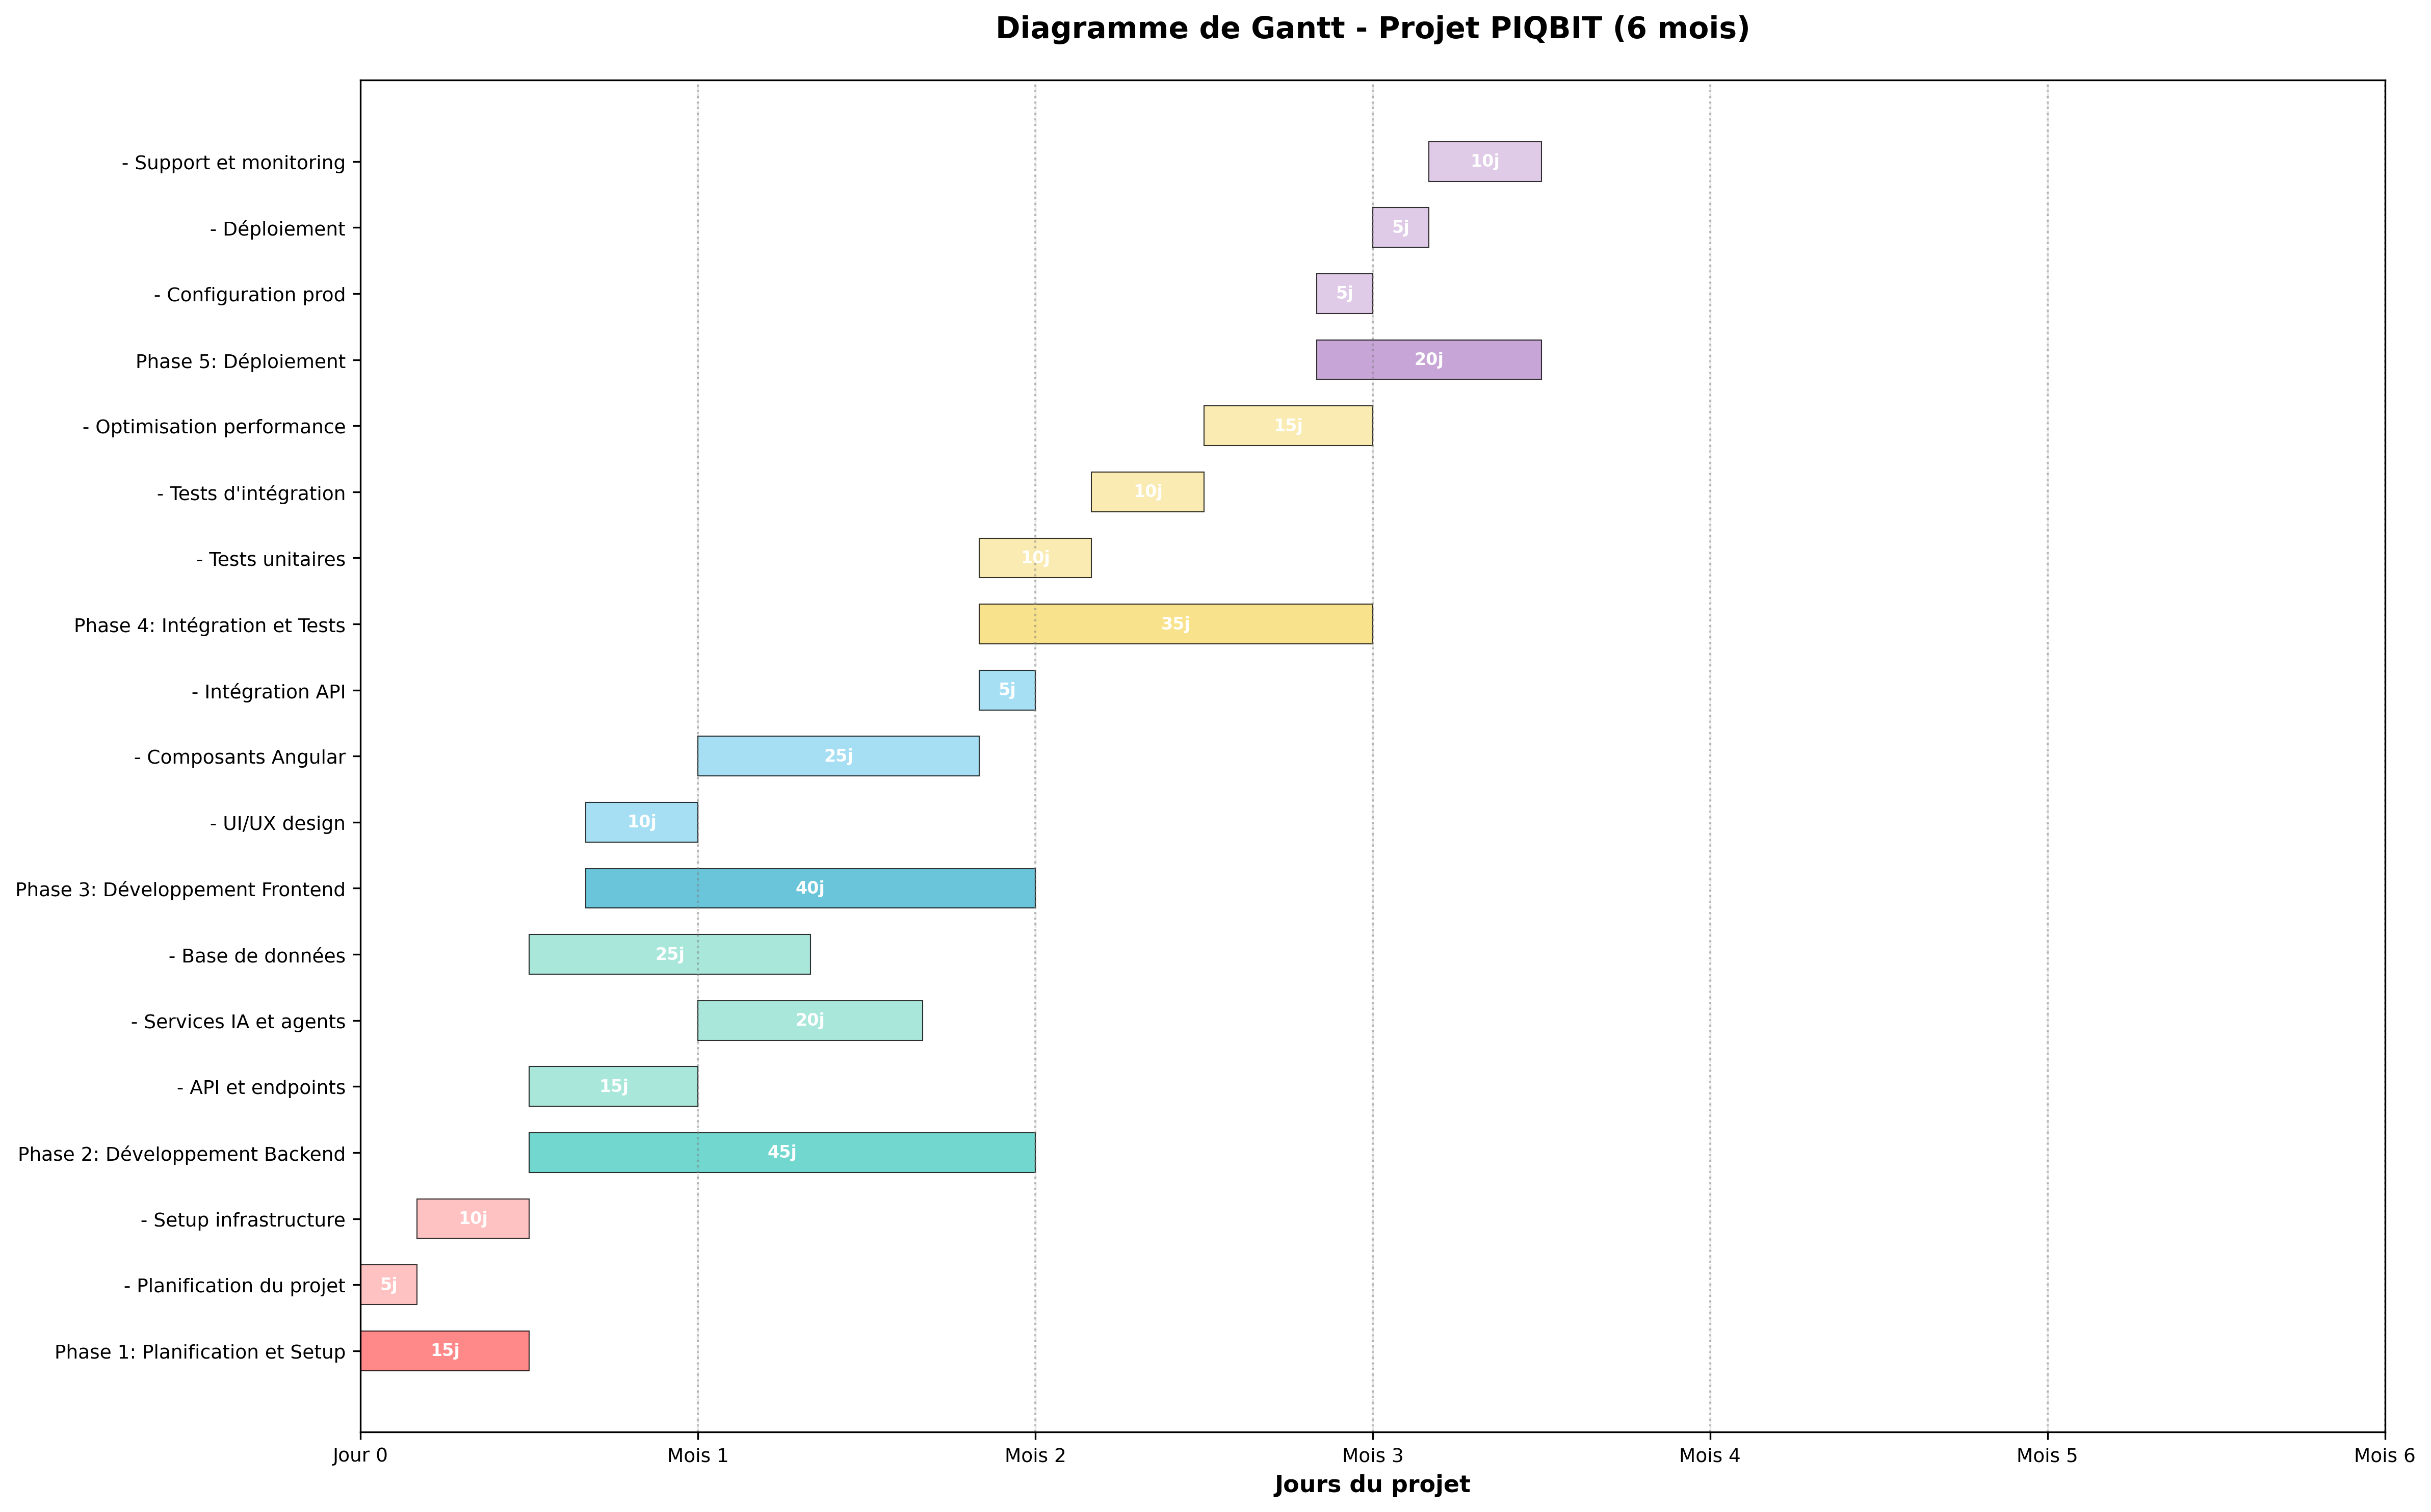
\includegraphics[width=\textwidth,keepaspectratio]{gantt_previsionnel}
  \caption[Diagramme de Gantt prévisionnel]{Diagramme de Gantt
    \textbf{prévisionnel} du projet, sur un horizon de 180 jours. Cette figure
    décrit une \emph{intention} de planification et non un déroulement
    constaté. Son découpage en cinq phases techniques ne coïncide pas avec les
    neuf phases fonctionnelles du tableau~\ref{tab:phases} : les deux
    plannings coexistent dans les sources du projet.}
  \label{fig:gantt_previsionnel}
\end{figure}

\champARemplir{Deux points à confirmer avant le dépôt. (1) Lequel des deux
découpages — neuf phases fonctionnelles ou cinq phases techniques — a
réellement guidé le travail ? Conserver celui-là et supprimer l'autre. (2) Si
vous avez tenu un suivi itératif (tableau de tâches, carnet, jalons datés),
l'ajouter ici ; sans trace, ne revendiquez pas de méthode agile — un jury
vérifie cette affirmation.}

\section{Conclusion du chapitre}
\label{sec:ctx_conclusion}

Ce chapitre a posé le contexte du recrutement assisté, montré que les
solutions existantes séparent la lecture du CV de la décision qu'elle devrait
éclairer, et formulé la problématique en termes d'automatisation
\emph{explicable}. Il a présenté le positionnement de PIQBIT, ses objectifs,
son périmètre et ses limites constatées.

Le chapitre suivant transforme ce cadrage en exigences : il identifie les
acteurs, formalise les exigences fonctionnelles et non fonctionnelles, décrit
les cas d'utilisation principaux et établit la base de traçabilité qui reliera
chaque exigence à son implémentation et à sa validation.
